%====================================================
%	CHAPTER 5 - Allocation
%====================================================
\chapter{Controller Allocation}
\label{ch:allocation}
%====================================================
Higher level attitude and position controllers (from Sec:\ref{sec:control.attitude} and Sec:\ref{sec:control.position} respectively) design a virtual control input $H(\vec{\mathbf{x}}_e,t)=\vec{\nu}_d=[\vec{F}_d~\vec{\tau}_d]^T$ to be applied by the vehicles actuators. The system's overactuation was previously described in Sec:\ref{sec:control.inputs}; this chapter aims to solve for explicit actuator positions from that virtual input. A simplified allocation block, reduced from Fig:\ref{fig:control-block},is shown in Fig:\ref{fig:allocation-block}.
\begin{figure}[htbp]
\vspace{-6pt}
\centering
\begin{subfigure}{0.48\textwidth}
\centering
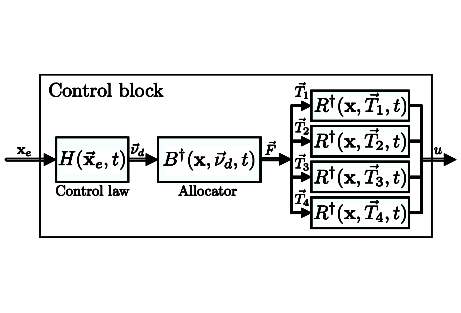
\includegraphics[width=\textwidth]{figs/allocator-block}
\vspace{-8pt}
\caption{Allocation block}
\label{fig:allocation-block}
\end{subfigure}
\begin{subfigure}{0.48\textwidth}
\centering
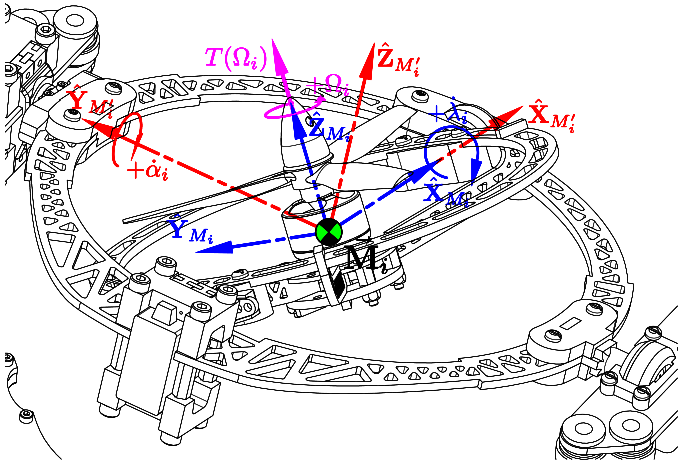
\includegraphics[width=\textwidth]{figs/force-redirect}
\vspace{-8pt}
\caption{Single thrust vector construction}
\label{fig:allocation-redirect}
\end{subfigure}
\vspace{-8pt}
\caption{Actuator allocation}
\vspace{-16pt}
\end{figure}
\par
A distribution rule is needed to \emph{allocate} out physical actuator positions $u_c\in\mathbb{U}$ to command that input $\vec{\nu}_c$, from Eq:\ref{eq:control-input}. As mentioned previously (pseudo) inversion based allocation requires an affine actuator effectiveness function; the allocator is abstracted to first solve for four thrust vectors which are applied by each motor module, Eq:\ref{eq:4.7}.
\begin{equation}\label{eq:5.1}
B^{\dagger}(\vec{\mathbf{x}},t)\vec{\nu}_d=\begin{bmatrix}
\vec{T}_1&\vec{T}_2&\vec{T}_3&\vec{T}_4
\end{bmatrix}^T
\end{equation}
Each 3-D thrust vector is then used to solve for each module's propeller speed in $\text{RPM}$ and both servo rotational positions in $\text{rad}$; undoing rotation applied by the motor module's structure in Fig:\ref{fig:allocation-redirect}.
\begin{equation}
u\cdot i = \begin{bmatrix}\Omega_i&\lambda_i&\alpha_i\end{bmatrix}^T=R^\dagger(\vec{\mathbf{x}},\vec{T}_i,t)~~~~\text{for}~i\in[1:4]
\end{equation}
%====================================================
\section{Generalized allocation}
\label{sec:allocation.slack}
%====================================================
Regular, unconstrained control allocation is solved as an optimization problem; shown in \cite{allocation,controlallocation}. The aim is to minimize deviation (\emph{slack}) between the virtual and commanded control inputs, $\vec{\nu}_d$ and $\vec{\nu}_c$ respectively. For the control law's virtual input $\vec{\nu}_d=\mathcal{H}(\vec{\mathbf{x}}_e,t)$ the optimization is then posed as:
\begin{equation}\label{eq:allocation-slack}
\underset{u\in\mathbb{U}^{m},~s\in\mathbb{R}^{n}}{min}\big(\norm{Q_s}\big)~~\text{such that}~~\vec{\nu}_d-\vec{\nu}_c=\mathcal{H}(\vec{\mathbf{x}}_e,t)-B(\vec{\mathbf{x}},t,u)\triangleq s
\end{equation}
Where $u\in\mathbb{U}^m$ is the dimension of the actuator set and $\vec{\mathbf{x}},~\vec{\nu}_d,~\vec{\nu}_c,~s$ are each the same dimension of virtual plant's input; $\in\mathbb{R}^{n}$ where $n$ is the degrees of freedom the state has. In this case $u\in\mathbb{U}^{12}$ for twelve actuators and $\vec{\mathbf{x}}\in\mathbb{R}^6$ for the 6-DOF rigid body.
\par
In Eq:\ref{eq:allocation-slack}, $\norm{Q_s}$ is the cost function prioritizing the slack variable; $s$. Typically that cost is just the $L_2$ norm of the slack. Overactuation asserts that there exists an entire set of suitable actuator values which are all solutions to Eq:\ref{eq:allocation-slack}. Solving for explicit actuator positions requires an introduction of a secondary cost function or control objective $J(\vec{\mathbf{x}},t,u)$ to refine the solution to of Eq:\ref{eq:allocation-slack}.
\begin{equation}\label{eq:allocation-problem}
\underset{u\in\mathbb{U}^{12},~s\in\mathbb{R}^{6}}{min}\big(||Q_s||+J(\vec{\mathbf{x}},u,t)\big)~~\text{such that}~~\mathcal{H}(\vec{\mathbf{x}}_e,t)-B(\vec{\mathbf{x}},u,t)=s
\end{equation}
That secondary control objective $J(\vec{\mathbf{x}},t,u)$ and its associated \emph{explicit} solution to Eq:\ref{eq:allocation-problem} is the subject of control allocation. Not much work has been done on overallocation for aerospace vehicles outside the field of satellite attitude control (Sec:\ref{subsubsec:intro.lit.control.allocation} for examples). Often satellites are over actuated for the sake of fault tolerance and redundancy\cite{FTCallocation,discreteFTC}. Actuator rate constraints can be further introduced such that $u$ is limited by $\Delta u$, constraining sequential actuator position changes.
\begin{multline}
\therefore\underset{u\in\mathbb{U}^{12},~s\in\mathbb{R}^6}{min}\big(||Q_s||+J(\vec{\mathbf{x}},u,t)\big)~~\text{s.t}~~\mathcal{H}(\vec{\mathbf{x}}_e,t)-B(\vec{\mathbf{x}},u,t)=s\\\text{and subject to}~~u=u_{n-1}+\Delta u,~\Delta u\in\mathbb{C}
\end{multline}
Allocation \emph{inverts} the effectiveness of the actuator set, $B(\vec{\mathbf{x}},u,t)$ in Eq:\ref{eq:control-effectiveness}, to find actuator positions which satisfy the virtual control input. Inverting the allocation requires a linear, multiplicative relationship with the effectiveness function; hence the abstraction layer which was introduced previously in Eq:\ref{eq:4.7}. The allocator effectiveness function, when abstracted to an affine matrix, reduces to:
\begin{equation}\label{eq:5.6}
\begin{bmatrix}
\vec{F}_d\\
\vec{\tau}_d
\end{bmatrix}={\nu}_d=\mathcal{H}(\vec{\mathbf{x}}_e,t)\Longleftrightarrow B(\vec{\mathbf{x}},u,t)=B'(\vec{\mathbf{x}},t)u_c=\vec{\nu}_c=\begin{bmatrix}
\vec{F}_c(\hat{u})\\
\vec{\tau}_c(\hat{u})
\end{bmatrix}
\end{equation}
The allocator commands an actuator setpoint $u_c$ which leads to actuator position estimates $\hat{u}_c=C(s)u_c$ from the actuator block transfer function defined in Eq:\ref{eq:actuator-constraints}. In Eq:\ref{eq:5.6} state dimensions are such that $(\vec{\nu}_d,\vec{\nu}_c)\in\mathbb{R}^n,\mathbb{U}\in\mathbb{R}^m,~\text{and}~B\in\mathbb{R}^{m\times n}$. That abstraction to a multiplicative $B'(\vec{\mathbf{x}},t)u_c$ in Eq:\ref{eq:4.7} makes addressing the allocation conceptually simpler, accommodating the use of inversion based allocation laws (Sec:\ref{subsec:allocation.allocators.inverse}-\ref{subsec:allocation.allocators.weightedinverse}).
%====================================================
\section{Thrust vector inversion}
\label{sec:allocation.inversion}
%====================================================
The rotation \emph{inversion} function $R^\dagger(\vec{\mathbf{x}},\vec{F}_i,t)$ to solve for physical actuator positions to be commanded $u_c(i)=[\Omega_i~\lambda_i~\alpha_i]^T$ is as yet undefined. Assuming for now there is some allocation rule that, from $\vec{\nu}_d$, designs well four decomposed stabilizing 3-D thrust vectors $\vec{T}_{1\rightarrow 4}$ to be actuated by each motor module. It then follows that each of those four thrust vectors relate to their individual associated actuator positions through a quaternion \emph{rotation}, not transformation:
\begin{subequations}
\begin{equation}\label{eq:quaternion-thrust-allocation}
\vec{T}_i= Q_{M_i}\otimes\vec{T}(\Omega_i)\otimes Q_{M_i}^*~~~~\in\mathcal{F}^b
\end{equation}
\vspace{-16pt}
\begin{equation}\label{eq:quaternion-thrust-allocation-expanded}
=Q_{z}(\sigma_i)Q_{y}(\alpha_i)Q_{x}(\lambda_i)\otimes \vec{T}(\Omega_i) \otimes Q_{x}^*(\lambda_i)Q_{y}^*(\alpha_i)Q_z^*(\sigma_i)
\end{equation}
Where each motor thrust vector, $\vec{T}(\Omega_i)$, is calculated using BEM thrust coefficients, Eq:\ref{eq:thrust-coefficient} with coefficients from Fig:\ref{fig:coeffs-plot}. The thrust produced is exclusively in the $\hat{Z}_{M_i}$ direction of the motor module's frame $\mathcal{F}^{M_i}$:
\begin{equation}
\vec{T}(\Omega_i)=\begin{bmatrix}
0&
0&
T(\Omega_i)
\end{bmatrix}^T=\begin{bmatrix}
0\\
0\\
C_T(J)\rho \Omega_i^2 D^4
\end{bmatrix}~~~~\in\mathcal{F}^{M_i}
\end{equation}
\end{subequations}
Seeing that quaternion rotation (or \emph{transformation}) operators change the reference frame but retains the vector operand's magnitude, it follows that $T(\Omega_i)$, and by extension the propeller speed $\Omega_i$, can be found:
\begin{subequations}
\begin{equation}
|\vec{T}_i|=\sqrt{\norm{\begin{bmatrix}T_x&T_y&T_z\end{bmatrix}}}=\sqrt{T_x^2+T_y^2+T_z^2}=|T(\Omega_i)|=|C_T(J)\rho\Omega_i^2D^4|
\end{equation}
\vspace{-14pt}
\begin{equation}
\rightarrow \Omega_i=\sqrt{\frac{|\vec{T}_i|}{C_T(J)\rho D^4}}=\sqrt{\frac{\sqrt{T_x^2+T_y^2+T_z^2}}{C_T(J)\rho D^4}}
\end{equation}
\end{subequations}
Reversing (or \emph{undoing}) that transformation from the motor module's frame to body frame in Eq:\ref{eq:quaternion-thrust-allocation}:
\begin{subequations}
\begin{equation}
\vec{T}(\Omega_i)=Q_{z}^*(\sigma_i)Q_{y}^*(\alpha_i)Q_{x}^*(\lambda_i)\otimes \vec{T}_i \otimes Q_{x}(\lambda_i)Q_{y}(\alpha_i)Q_z(\sigma_i)~~~~\in\mathcal{F}^{M_i}
\end{equation}
\vspace{-14pt}
\begin{equation}\label{eq:thrust-vector-motor-transformation}
\rightarrow \vec{T}(\Omega_i)=Q_{M_i}^*\otimes \vec{T}_i \otimes Q_{M_i}~~~~\in\mathcal{F}^{M_i}
\end{equation}
\end{subequations}
Knowing only $\vec{T}(\Omega_i)$ and $\vec{T}_i$ in the motor frame and body frame respectively requires solving for a quaternion which relates the two. If both vectors are of unit length, $\breve{T}_i$ and $\breve{T}(\Omega_i)$; then the following relationship can be used to construct a relative quaternion:
\begin{subequations}
\begin{equation}
\breve{T}_i\triangleq\frac{\vec{T}_i}{|\vec{T}_i|}=\frac{\vec{T}_i}{\sqrt{T_x^2+T_y^2+T_z^2}}~~~~\in\mathcal{F}^b
\end{equation}
\vspace{-8pt}
\begin{equation}
\breve{T}(\Omega_i)\triangleq\frac{\vec{T}(\Omega_i)}{|\vec{T}(\Omega_i)|}=\frac{\vec{T}(\Omega_i)}{|C_T(J)\rho\Omega^2 D^4|}=\begin{bmatrix}
0 & 0 & 1
\end{bmatrix}^T~~~~\in\mathcal{F}^{M_i}
\end{equation}
\vspace{-4pt}
\begin{equation}\label{eq:vector-quaternion}
\therefore Q_{M_i}=\begin{bmatrix}
q_0\\
\vec{q}
\end{bmatrix}
=
\begin{bmatrix}
1+\breve{T}_i\cdot \breve{T}(\Omega_i)\\
-\breve{T}_i\times\breve{T}(\Omega_i)
\end{bmatrix}
\end{equation}
\end{subequations}
Where Eq:\ref{eq:vector-quaternion} is a quaternion operator's definition, rotating a vector around a single Euler axis, Eq:\ref{eq:quaternion-euler-axis}, when applied to two unit vectors. That quaternion can indeed be used to solve for relative pitch, roll and yaw Euler angles (see App:\ref{app:equations.quaternions}). However, Eq:\ref{eq:vector-quaternion} solves for the \textbf{shortest rotational path} between the two vectors, a sequenced Z-Y-X rotation is by no means the shortest possible rotation. Associated $[\phi,~\theta,~\psi]^T$ solutions to Eq:\ref{eq:app-quaternion-eule} are of no consequence when solving for the sequentially applied rotation angles $[\lambda_i,~\alpha_i,~\sigma_i]^T$, where $\sigma_i$ is a known orthogonal multiplicate. Furthermore, when considering a sequenced Z-Y-X quaternion, angular operands cannot be extracted without applying significantly complex trigonometric inversions:
\begin{subequations}
\begin{equation}
Q_b\triangleq\begin{bmatrix}
cos\frac{\psi}{2}\\
0\\
0\\
sin\frac{\psi}{2}
\end{bmatrix}
\otimes
\begin{bmatrix}
cos\frac{\theta}{2}\\
0\\
sin\frac{\theta}{2}\\
0
\end{bmatrix}
\otimes
\begin{bmatrix}
cos\frac{\phi}{2}\\
sin\frac{\phi}{2}\\
0\\
0
\end{bmatrix}
=
\begin{bmatrix}
c\frac{\psi}{2}c\frac{\theta}{2}c\frac{\phi}{2}+s\frac{\psi}{2}s\frac{\theta}{2}s\frac{\phi}{2}\\
c\frac{\psi}{2}c\frac{\theta}{2}s\frac{\phi}{2}-s\frac{\psi}{2}s\frac{\theta}{2}c\frac{\phi}{2}\\
c\frac{\psi}{2}s\frac{\theta}{2}c\frac{\phi}{2}+s\frac{\psi}{2}c\frac{\theta}{2}s\frac{\phi}{2}\\
s\frac{\psi}{2}c\frac{\theta}{2}c\frac{\phi}{2}-c\frac{\psi}{2}s\frac{\theta}{2}s\frac{\phi}{2}
\end{bmatrix}
=
\begin{bmatrix}
q_0\\
q_x\\
q_y\\
q_z
\end{bmatrix}
=
\begin{bmatrix}
q_0\\
\vec{q}
\end{bmatrix}
\end{equation}
\vspace{-4pt}
\begin{equation}
\therefore\vec{T}_i=
\begin{bmatrix}
c\frac{\psi}{2}c\frac{\theta}{2}c\frac{\phi}{2}+s\frac{\psi}{2}s\frac{\theta}{2}s\frac{\phi}{2}\\
c\frac{\psi}{2}c\frac{\theta}{2}s\frac{\phi}{2}-s\frac{\psi}{2}s\frac{\theta}{2}c\frac{\phi}{2}\\
c\frac{\psi}{2}s\frac{\theta}{2}c\frac{\phi}{2}+s\frac{\psi}{2}c\frac{\theta}{2}s\frac{\phi}{2}\\
s\frac{\psi}{2}c\frac{\theta}{2}c\frac{\phi}{2}-c\frac{\psi}{2}s\frac{\theta}{2}s\frac{\phi}{2}
\end{bmatrix}
\otimes
\vec{T}(\Omega_i)
\otimes
\begin{bmatrix}
s\frac{\psi}{2}s\frac{\theta}{2}s\frac{\phi}{2}+c\frac{\psi}{2}c\frac{\theta}{2}c\frac{\phi}{2}\\
s\frac{\psi}{2}s\frac{\theta}{2}c\frac{\phi}{2}-c\frac{\psi}{2}c\frac{\theta}{2}s\frac{\phi}{2}\\
-c\frac{\psi}{2}s\frac{\theta}{2}c\frac{\phi}{2}-s\frac{\psi}{2}c\frac{\theta}{2}s\frac{\phi}{2}\\
c\frac{\psi}{2}s\frac{\theta}{2}s\frac{\phi}{2}-s\frac{\psi}{2}c\frac{\theta}{2}c\frac{\phi}{2}
\end{bmatrix}
\end{equation}
\end{subequations}
Instead; returning to rotation matrices to resolve the inverse transformation and reiterating that Euler angle equivalents for the servos are; $[\phi,~\theta,~\psi]^T\iff [\lambda_i,~\alpha_i,~\sigma_i]^T$. The rotation matrix transformation from $\mathcal{F}^{M_i}$ to $\mathcal{F}^b$, analogous to Eq:\ref{eq:thrust-vector-motor-transformation}, is:
\begin{subequations}
\begin{equation}
\vec{T}_i=R_z(\sigma_i)R_y(\alpha_i)R_x(\lambda_i)\vec{T}(\Omega_i)~~~~\in\mathcal{F}^b
\end{equation}
\vspace{-12pt}
\begin{equation}
=\begin{bmatrix}
c\sigma_i & -s\sigma_i & 0\\
s\sigma_i & c\sigma_i & 0\\
0 & 0 & 1 
\end{bmatrix}
\begin{bmatrix}
c\alpha_i & 0 & s\alpha_i\\
0 & 1 & 0\\
-s\alpha_i & 0 & c\alpha_i
\end{bmatrix}
\begin{bmatrix}
1 & 0 & 0\\
0 & c\lambda_i & -s\lambda_i\\
0 & s\lambda_i & c\lambda_i
\end{bmatrix}\vec{T}(\Omega_i)
\end{equation}
\vspace{-4pt}
\begin{equation}
\therefore\vec{T}_i=\begin{bmatrix}
c\sigma_i c\alpha_i & c\sigma_i s\alpha_i s\lambda_i - s\sigma_i c\lambda_i & c\sigma_i s\alpha_i c\lambda_i + s\sigma_i s\lambda_i\\
s\sigma_i c\alpha_i & s\sigma_i s\alpha_i s\lambda_i + c\sigma_i c\lambda_i & s\sigma_i s\alpha_i c\lambda_i - c\sigma_i s\lambda_i\\
-s\alpha_i & c\alpha_i s\lambda_i & c\alpha_i c\lambda_i
\end{bmatrix}
\begin{bmatrix}
0\\
0\\
T(\Omega_i)
\end{bmatrix}
\end{equation}
Where $\sigma_i$ is an orthogonal multiple applying a rotation about the $\hat{Z}_b$ axis (Fig:\ref{fig:body-frame}). Because the thrust vector $\vec{T}(\Omega_i)$ is only in the motor frame's $\hat{Z}_{M_i}$ direction, solving for servo angles is simplified.
\begin{equation}\label{eq:rotation-inverse}
\rightarrow
\begin{bmatrix}
T_x\\
T_y\\
T_z
\end{bmatrix}
=\begin{bmatrix}
s\sigma_i s\lambda_i + c\sigma_i s\alpha_i c\lambda_i\\
s\sigma_i s\alpha_i c\lambda_i - c\sigma_i s\alpha_i\\
c\alpha_i c\lambda_i
\end{bmatrix}
T(\Omega_i)~~~~\in\mathcal{F}^{b}
\end{equation}
\end{subequations}
Eq:\ref{eq:rotation-inverse} then reduces further with $R_z(\sigma_i)$ rotation matrices already defined in Eq:\ref{eq:motor-module-rotation.b}. The following four trigonometric relationships exist for each motor module respectively:
\begin{equation}
\begin{bmatrix}
T_x\\
T_y\\
T_z
\end{bmatrix}
=
\begin{bmatrix}
\begin{bmatrix}
s\alpha_1 c\lambda_1\\
-s\lambda_1 \\
c\alpha_1 c\lambda_1
\end{bmatrix}
,
\begin{bmatrix}
s\lambda_2\\
s\alpha_2 c\lambda_2\\
c\alpha_2 c\lambda_2
\end{bmatrix}
,
\begin{bmatrix}
-s\alpha_3 c\lambda_3\\
s\lambda_3\\
c\alpha_3 c\lambda_3
\end{bmatrix}
,
\begin{bmatrix}
-s\lambda_4\\
-s\alpha_4 c\lambda_4\\
c\alpha_4 c\lambda_4
\end{bmatrix}
\end{bmatrix}T(\Omega_{1\rightarrow 4})
\end{equation}
It is then a simple trigonometric inversion to solve for both $\lambda_i$ and $\alpha_i$. For the example case of $i=1$, the sequel holds true and can similarly be extended to the remaining modules. Firstly using $T(\Omega_i)=||\vec{T}_i||$ and implementing a four quadrant secondary arctangent2 function. Wherein $arctan2(x,y)$ is the four-quadrant tangent inverse\cite{atan2}, producing the principle argument of the complex operands:
\begin{equation}
arctan2(x,~y)=PR~arg(x+y\hat{\imath})=Arg(x+y\hat{\imath})
\end{equation}
The use of a full quadrature arctangent function is to find solutions for Euler angles that are not only acute. Each inverse would otherwise need generalized reciprocal solutions with parity checks to establish which quadrant the angle occurs in. Furthermore exploiting the fact that $arctan(x)\equiv arcsin(x/\sqrt{1-x^2})$:
\begin{subequations}
\begin{equation}
\lambda_i =  arctan2\bigg(-T_y,~\sqrt{||\vec{T}_i||^2-T_y^2}\hspace{2pt}\bigg)
\end{equation}
\vspace{-12pt}
\begin{equation}
\alpha_i = arctan2\big(T_x,~T_z\hspace{2pt}\big)
\end{equation}
\end{subequations}
Therefore, the secondary component of the control allocation block, $R^\dagger(\vec{\mathbf{x}},\vec{T}_i,t)$ from Fig:\ref{fig:control-block} is then summarized as a single rotation inversion function (in this case for $i=1$):
\begin{equation}\label{eq:allocator-inersion}
\begin{bmatrix}
\Omega_1\\
\lambda_1\\
\alpha_1
\end{bmatrix}
=
R^\dagger(\mathbf{x},\vec{T}_1,t)\triangleq
\begin{bmatrix}
\Big(\sqrt{T_x\text{}^2+T_y\text{}^2+T_z\text{}^2}/C_T(J)\rho D^4\Big)\text{}^{\frac{1}{2}}\\
atan2(-T_y\text{}^2,~||\vec{T}_1||\sqrt{||\vec{T}_1||\text{}^2-T_y\text{}^2})\\
atan2(T_x,~T_z||\vec{T}_1||)
\end{bmatrix}
\end{equation}
Rotation inversion equations for the remaining motor modules are included in App:\ref{app:equations.inversion}. The complete control block only requires one final abstracted allocation algorithm, $B^\dagger(\mathbf{x},\vec{\nu}_d,t)$; which is now addressed\ldots
%====================================================
\section{Allocators}
\label{sec:allocation.allocators}
%====================================================
%====================================================
\subsection{Pseudo Inverse Allocator}
\label{subsec:allocation.allocators.inverse}
%====================================================
The simplest control allocation solution to Eq:\ref{eq:allocation-problem} stems from what is categorized as \emph{inversion}, based on controller effort optimization \cite{allocation}. The requirements for inversion based allocation is that the effectiveness function $B(\vec{\mathbf{x}},u,t)$ is a linear relationship which can be abstracted to $B'(\vec{\mathbf{x}},t)u$. The objective is for some commanded control input $\vec{\nu}_c$ to find an inverted matrix $B^\dagger(\vec{\mathbf{x}},t)$ such that for a virtual control input $\vec{\nu}_d$:
\begin{subequations}\label{eq:inversion-identity}
\begin{equation}
\vec{\nu}_d=H(\vec{\mathbf{x}}_e,t)\iff B'(\vec{\mathbf{x}},t)u_c=\vec{\nu}_c
\end{equation}
\vspace{-16pt}
\begin{equation}
 \rightarrow u_c = B^\dagger(\vec{\mathbf{x}},t)\vec{\nu}_d
\end{equation}
\vspace{-12pt}
\begin{equation}
\therefore \vec{\nu}_c=B'(\vec{\mathbf{x}},t)B^\dagger(\vec{\mathbf{x}},t)\vec{\nu}_d
\end{equation}
Where the inverse namesake is as a result of the identity condition for both the effectiveness matrix $B'(\vec{\mathbf{x}},t)$ and it's inverse $B^\dagger(\vec{\mathbf{x}},t)$:
\begin{equation}
B'(\vec{\mathbf{x}},t)B^\dagger(\vec{\mathbf{x}},t)=\mathbb{I}_{m\times m}
\end{equation}
{\color{Gray}\emph{Or more generally, and without the dependency of the affine linearity:}}
\begin{equation}
\color{Gray} u_c=B^\dagger(\vec{\mathbf{x}},\vec{\nu}_d,t)
\end{equation}
\end{subequations}
In Eq:\ref{eq:inversion-identity}, the multiplicative effectiveness matrix $B'(\vec{\mathbf{x}},t)$ has the dimension $\in\mathbb{R}^{m\times n}$. In the case of overallocation there are more actuators than degrees of freedom, or that $m>n$ for $u\in\mathbb{R}^{m}$ and $\vec{\mathbf{x}}\in\mathbb{R}^{n}$. That implies that $B'$ has full rank, therefore finding the inversion of $B^\dagger(\mathbf{x},t)$ is not trivial. Choosing the secondary control objective, $J(\vec{\mathbf{x}},u,t)$ in Eq:\ref{eq:allocation-problem}, to be a quadratic cost function; actuator positions $u_c$ to be commanded can be solved as a linear least squares problem. The quadratic least squares optimization aims to minimize controller effort (\emph{magnitude}):
\begin{equation}\label{eq:allocation-quadratic}
J(\vec{\mathbf{x}},u_c,t)=\underset{u_c\in\mathbb{U}}{min}\frac{1}{2}\big(u_c-u_p\big)^TW\big(u_c-u_p)~~\text{such that}~~\vec{\nu}_c=B'(\vec{\mathbf{x}},t)u_c
\end{equation}
The least squares solution, \cite{matrixcomputations}, to Eq:\ref{eq:allocation-quadratic} then minimizes the commanded actuator actuator effort, $\norm{u}_c$. This means that thrusts $\norm{\vec{T}_{1\rightarrow 4}}$ from Eq:\ref{eq:5.1} are minimized. The magnitude of each thrust vector commanded to a motor module is affected by the propeller's rotational speed $\Omega_i$. Effectively this results in an allocator that prioritizes pitching or rolling both servos $\lambda_i$ and $\alpha_i$ over adjusting the propeller's velocity. 
\par
The positive symmetrical weighting matrix $W$ in Eq:\ref{eq:allocation-quadratic} biases certain actuators (thrust components in this case) and creates its own class of inversion allocator, presented in Sec:\ref{subsec:allocation.allocators.weightedinverse}. Similarly $u_p$ is the preferred actuator value to which the system naturally tends; discussed in Sec:\ref{subsec:allocation.allocators.norminverse}. For an inversion matrix $B^\dagger(\vec{\mathbf{x}},t)$ actuator thrust components are found:
\begin{subequations}\label{eq:inversion}
\begin{equation}
\underset{u\in\mathbb{U}}{\begin{bmatrix}
\vec{T}_{1\rightarrow 4}
\end{bmatrix}}=\Big(\mathbb{I}_{m\times m}-CB(\vec{\mathbf{x}},t)\Big)\vec{T}_p+C\vec{\nu}_d
\end{equation}
\vspace{-6pt}
\begin{equation}
C=W^{-1}B^T(\vec{\mathbf{x}},t)\big(B(\vec{\mathbf{x}},t)W^{-1}B^T(\vec{\mathbf{x}},t)\big)^{-1}
\end{equation}
\end{subequations}
Where $\vec{T}_p\in\mathbb{R}^{1\times 12}$ are preferred thrust component values. The solution in Eq:\ref{eq:inversion} is a \emph{generalized inverse} with weighted actuators components and preferred values. In the case where no weightings nor preferred actuator values are specified, $W=\mathbb{I}_{n\times n}$ and $u_p=\vec{T}_p=\vec{0}$, the solution reduces:
\begin{subequations}\label{eq:pseudo-inversion}
\begin{equation}
\vec{T}_{1\rightarrow 4}=B^T(\vec{\mathbf{x}},t)\big(B(\vec{\mathbf{x}},t).B^T(\vec{\mathbf{x}},t)\big)^{-1}\vec{\nu}_d
\end{equation}
\vspace{-15pt}
\begin{equation}
=B^\ddagger(\vec{\mathbf{x}},t) \vec{\nu}_d~~,B^\ddagger\in\mathbb{R}^{6\times 12}
\end{equation}
\end{subequations}
The simplified case in Eq:\ref{eq:pseudo-inversion} is termed a Moore-Penrose or pseudo-inversion of the actuator effectiveness matrix $B'(\vec{\mathbf{x}},t)$, \cite{moorepenrose}. Pseudo-inversion is the simplest allocation rule to implement, in most cases controller effort optimization is a satisfactory constraint without any additional weights or preferred values. For an effectiveness $B'(\vec{\mathbf{x}},t)$ matrix defined in Eq:\ref{eq:4.7}, the pseudo-inversion is:
\begin{subequations}\label{eq:pseudo-bmatrix}
\begin{equation}\label{eq:pseudo-bmatrix.a}
B'(\vec{\mathbf{x}},t)=\begin{bmatrix}
\mathbb{I}_{3\times 3} & \mathbb{I}_{3\times 3} & \mathbb{I}_{3\times 3} & \mathbb{I}_{3\times 3}\\
[\vec{L}_1]_\times & [\vec{L}_2]_\times & [\vec{L}_3]_\times & [\vec{L}_4]_\times
\end{bmatrix}~~~~\in\mathbb{R}^{12\times 6}
\end{equation}
\vspace{-2pt}
\begin{equation}
\therefore \vec{T}_{1\rightarrow 4}=B^T\big(B.B^T\big)^{-1}\vec{\nu}_d=B^{\ddagger}(\vec{\mathbf{x}},t)\vec{\nu}_d
\end{equation}
Recalling that each motor modules displacement is  at a distance $L_{arm}=195.16~\text{mm}$ from Fig:\ref{fig:inertia-frame}. Then each module has a vector $\vec{L}_{1,3}=\begin{bmatrix}
\pm 195.16 & 0 & 0
\end{bmatrix}^T$ and $\vec{L}_{2,4}=\begin{bmatrix}
0 & \pm 195.16 & 0
\end{bmatrix}$. Each cross product vector in Eq:\ref{eq:pseudo-bmatrix.a} is defined from Eq:\ref{eq:cross-product-matrix} as:
\begin{equation}
\big[\vec{L}_i\big]_\times\triangleq\begin{bmatrix}
0 & -L_z & L_y\\
L_z & 0 & -L_x\\
-L_y & L_x & 0
\end{bmatrix}
\end{equation}
The numeric and constant pseudo-inverse matrix is then:
\begin{equation}\label{eq:pseudo-bmatrix.c}
\therefore B^\ddagger(\vec{\mathbf{x}},t)=
\begin{bmatrix}
\frac{1}{4} & 0 & 0 & 0 & 0 & 0\\
0 & \frac{1}{4} & 0 & 0 & 0 & \frac{1}{4L}\\
0 & 0 & \frac{1}{4} & 0 & \frac{-1}{2L} & 0\\
\frac{1}{4} & 0 & 0 & 0 & 0 & \frac{-1}{4L}\\
0 & \frac{1}{4} & 0 & 0 & 0 & 0\\
0 & 0 & \frac{1}{4} & \frac{1}{2L} & 0 & 0\\
\frac{1}{4} & 0 & 0 & 0 & 0 & 0\\
0 & \frac{1}{4} & 0 & 0 & 0 & \frac{-1}{4L}\\
0 & 0 & \frac{1}{4} & 0 & \frac{1}{2L} & 0\\
\frac{1}{4} & 0 & 0 & 0 & 0 & \frac{1}{4L}\\
0 & \frac{1}{4} & 0 & 0 & 0 & 0\\
0 & 0 & \frac{1}{4} & \frac{-1}{2L} & 0 & 0
\end{bmatrix}
\end{equation}
\begin{equation}
=\begin{bmatrix*}[r]
0.250 & 0.000 & 0.000 & 0.000 & 0.000 & 0.000\\
0.000 & 0.250 & 0.000 & 0.000 & 0.000 & 0.250\\
0.000 & 0.000 & 0.250 & 0.000 & -2.562 & 0.000\\
0.250 & 0.000 & 0.000 & 0.000 & 0.000 & -1.281\\
0.000 & 0.250 & 0.000 & 0.000 & 0.000 & 0.000\\
0.000 & 0.000 & 0.250 & 2.562 & 0.000 & 0.000\\
0.250 & 0.000 & 0.000 & 0.000 & 0.000 & 0.000\\
0.000 & 0.250 & 0.000 & 0.000 & 0.000 & -1.281\\
0.000 & 0.000 & 0.250 & 0.000 & 2.562 & 0.000\\
0.250 & 0.000 & 0.000 & 0.000 & 0.000 & 1.281\\
0.000 & 0.250 & 0.000 & 0.000 & 0.000 & 0.000\\
0.000 & 0.000 & 0.250 & -2.562 & 0.000 & 0.000
\end{bmatrix*}
\end{equation}
\end{subequations}
Pseudo-inversion allocation guarantees that $\vec{T}_{1\rightarrow 4}=B^\dagger(\vec{\mathbf{x}},t)\vec{\nu}_d$ produces a feasible set of control thrust vectors $\vec{T}_{1\rightarrow 4}$ for some virtual control input $\vec{\nu}_d=\mathcal{H}(\vec{\mathbf{x}}_e,t)$.  Those thrust vectors, each $\vec{T}_{i}$, is then solved for as explicit actuator positions $[\Omega_i,\lambda_i,\alpha_i]^T=R^\dagger(\mathbf{x},\vec{T}_i,t)$ using Eq:\ref{eq:allocator-inersion}. That constructs an actuator matrix $u_c\in\mathbb{U}\in\mathbb{R}^{12}$ which will physically command $\vec{\nu}_c=B(\vec{\mathbf{x}},t)u_c$. 
\par
The actuator's effectiveness matrix $B(\vec{\mathbf{x}},t,u)$ does not necessarily have to be static (or affine) with respect to either the state vector $\vec{\mathbf{x}}$ or time $t$. However it was abstracted to such a static relationship to simplify the actuation process. Allocation in Eq:\ref{eq:pseudo-bmatrix} is the most simplified case of the least squares quadratically optimized equation for Eq:\ref{eq:allocation-problem} and is used as the base reference allocation law.
\par
The direct (\emph{pseudo}) inversion solution ensures the commanded virtual control input is met and that acutators are not necessarily saturated. In certain cases it may be desired to completely saturate certain actuators before exploiting other actuator plant inputs. That would entail an iterative \emph{daisy chaining} allocation to be performed numerically online, enforcing saturation for atleast some actuators and achievement of control objectives, \cite{allocation}. Such an approach is avoided here as completely saturating any actuator is not desirable; moreover online allocation is outside the scope of applied allocation rules here, static explicit allocation rules are only investigated\ldots
%====================================================
\subsection{Priority Norm Inverse Allocator}
\label{subsec:allocation.allocators.norminverse}
%====================================================
Choosing a preferred actuator position from Eq:\ref{eq:allocation-problem} produces what is termed as a \emph{priority norm} allocator. Specifically when $u_p=\vec{T}_p\not=\vec{0}\in\mathbb{U}$. An obvious choice for that value are the conditions required for stable hovering, those which simply keep the quadcopter airborne. The desired effect is that the controller constantly tends towards stability with small first and second order rates. There are, however, some intricacies which must be discussed with respect to what hovering conditions are.
\par
For a vehicle with a weight $m_b$ a net gravitational force acts on the vehicle through its center of gravity in the inertial frame; $-m_b\vec{G}_I\in\mathcal{F}^I$. Assuming torques produced by the eccentric gravitational center (Eq:\ref{eq:consolidated-grav-torque}) at steady state are going to be constant, hovering conditions are then simply:
\begin{equation}\label{eq:hover}
\vec{\nu}_I=
\begin{bmatrix}
\vec{F}_p\hspace{3pt}\\
\vec{\tau}_p\hspace{3pt}
\end{bmatrix}
=
\begin{bmatrix}
m_b\vec{G}_I\hspace{3pt}\\
\Delta C.G \times m_b\vec{G}_I
\end{bmatrix}~~~~\in\mathcal{F}^I
\end{equation}
\par
If the hover conditions are taken with respect to the inertial frame as in Eq:\ref{eq:hover} then the resultant preferred actuator positions are independent from the body's current or desired attitude setpoint. The control loop then naturally tends towards a rest state attitude at $Q_d=[1~\vec{0}\hspace{1pt}]^T$ with $\vec{\nu}_I\equiv\vec{\nu}_b$. The free body diagram in Fig:\ref{fig:hover-inertial} shows the tendency toward hovering conditions in the inertial frame.
\begin{figure}[htbp]
\centering
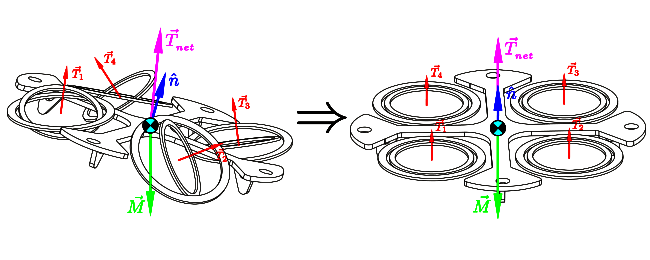
\includegraphics[width=\textwidth]{figs/hover-inertial}
\caption{Hover conditions W.R.T the inertial frame $\mathcal{F}^I$}
\label{fig:hover-inertial}
\vspace{-20pt}
\end{figure}
\par
Alternatively the hover conditions can be defined with respect to the body frame, being a function of the body's attitude.(Fig:\ref{fig:hover-body}). The difference is that the body's preferred actuator positions are dependent on each instantaneous orientation. That attitude stays constant whilst the actuators are redirected to produce inertial hovering conditions; irrespective of the attitude. The preferred hovering conditions are then always dependent on the commanded attitude trajectory.
\begin{subequations}\label{eq:hover-body}
\begin{equation}
m_b\vec{G}_b\triangleq m_b Q_b^*\otimes\vec{G}_I\otimes Q_b~~~~\in\mathcal{F}^{b}
\end{equation}
\vspace{-12pt}
\begin{equation}
\vec{\nu}_b=
\begin{bmatrix}
\vec{F}_p\hspace{3pt}\\
\vec{\tau}_p\hspace{3pt}
\end{bmatrix}
=\begin{bmatrix}
m_b\vec{G}_b\\
\Delta C.G \times m_b\vec{G}_b
\end{bmatrix}~~~~\in\mathcal{F}^b
\end{equation}
\end{subequations}
\par
\begin{figure}[htbp]
\vspace{-12pt}
\centering
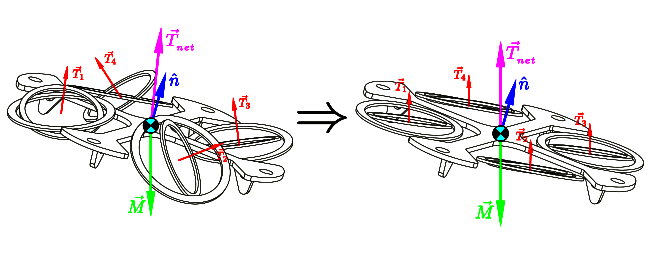
\includegraphics[width=\textwidth]{figs/hover-body}
\vspace{-12pt}
\caption{Hover conditions W.R.T the body frame $\mathcal{F}^b$}
\label{fig:hover-body}
\vspace{-8pt}
\end{figure}
\par
Specific module thrust values are then solved for using Eq:\ref{eq:hover} and Eq:\ref{eq:hover-body} with pseudo inversion from Eq:\ref{eq:pseudo-inversion}. The two solutions are then as follows:
\begin{subequations}\label{eq:priority-norm}
\begin{equation}\label{eq:priority-norm-inertial}
\vec{T}_p^I=B^\dagger(\mathbf{x},\vec{\nu}_I,t)~~\text{for hover in Fig\ref{fig:hover-inertial}}
\end{equation}
\vspace{-15pt}
\begin{equation}\label{eq:priority-norm-body}
\vec{T}_p^b=B^\dagger(\mathbf{x},\vec{\nu}_b,t)~~\text{for hover in Fig:\ref{fig:hover-body}}
\end{equation}
\end{subequations}
Both actuator matrices are then applied to Eq:\ref{eq:inversion} and could be combined with a non-diagonal weighting matrix.
\begin{subequations}
\begin{equation}
\underset{u\in\mathbb{U}}{\begin{bmatrix}\vec{T}_{1\rightarrow 4}\end{bmatrix}}=(\mathbb{I}_{m\times m}-CB(\vec{\mathbf{x}},t)\big)\vec{T}_p+C\vec{\nu}_d
\end{equation}
\vspace{-10pt}
\begin{equation}
C=W^{-1}B^T(\vec{\mathbf{x}},t)\big(B(\vec{\mathbf{x}},t)W^{-1}B^T(\vec{\mathbf{x}},t)\big)^{-1}
\end{equation}
\end{subequations}
Then applying the the inverse rotation operator $R^\dagger$ from Eq:\ref{eq:allocator-inersion} to the above solves for propeller speeds and servo rotational positions in both respective cases. The physical consequences of either preferred hovering codition and its associated actuator positions are demonstrated in simulation in Sec:\ref{sec:simulation.allocator}. Priority actuator positions are not tested together with weighting matrices, the two are compared independently\ldots
%====================================================
\subsection{Weighted Pseudo Inverse Allocator}
\label{subsec:allocation.allocators.weightedinverse}
%====================================================
Adding weights to the inversion in Eq:\ref{eq:inversion} but regarding preferred actuator positions as negligible, or that $\vec{T}_p=\vec{0}$, produces a \emph{weighted pseudo inverse} allocator. The positive symmetrical weighting matrix is square with respect to the actuator dimension; here $W\in\mathbb{R}^{12\times 12}$, but more generally $W\in\mathbb{R}^{m\times m}$. The Moore-Penrose inversion (Eq:\ref{eq:pseudo-inversion}) assumes that each actuator is weighted equally. Such a case makes the weighting matrix $W$ purely diagonal; $W_\ddagger\triangleq\mathbb{I}_{m\times m}$. 
\par
A weighting matrix could change adaptively over time or state dependency; following control faults or actuator deterioration. The control objective of a weighted inversion is to design the explicit weighting coefficients as per some preferred heuristic or optimization. Adaptive weighting is not considered or discussed as that is out of the scope for this work and pertains more to FTC\cite{FTCallocation}.
\par
\begin{figure}[htbp]
\vspace{-6pt}
\centering
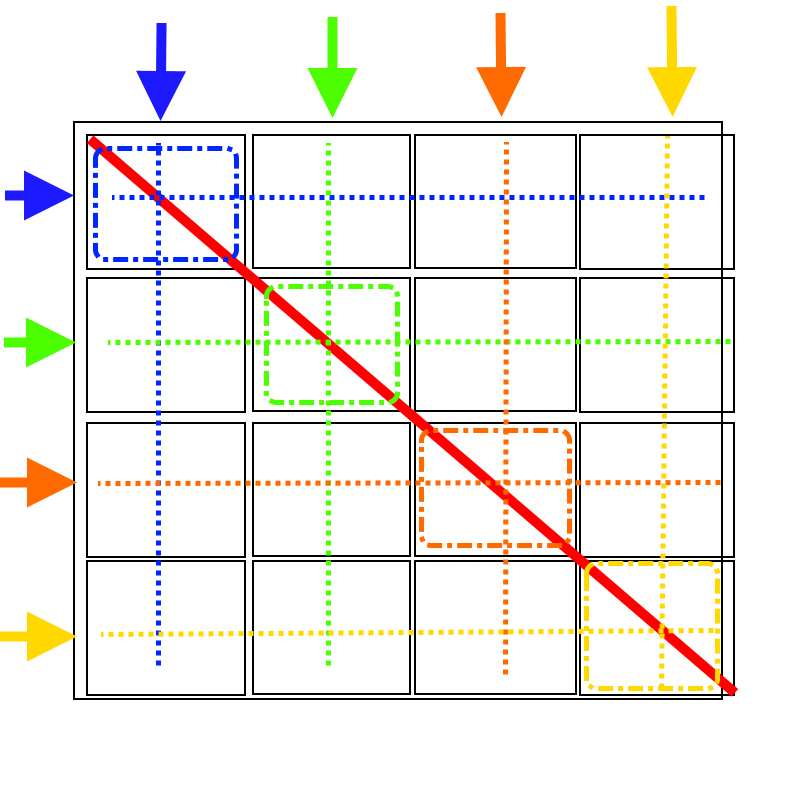
\includegraphics[width=0.6\textwidth]{figs/weighted-matrix}
\label{fig:weighted-matrix}
\vspace{-6pt}
\caption{Weighting matrix biasing}
\vspace{-6pt}
\end{figure}
Each coefficient in $W$ determines how the least squares solution to Eq:\ref{eq:allocation-problem} preferentially biases a particular actuator; here the weighting matrix's divisions correlate to mixed module thrust vectors. Each $3\times 3$ diagonal group for $W_{1\rightarrow 4}$ relate to individual thrust component biasing ($T_{ix},T_{iy},T_{iz}$) whilst off-centre $3\times 3$ groupings mix separate thrust terms $\vec{T}_{1\rightarrow 4}$. 
\par
Pseudo-inversion exactly matches the virtual control input $\vec{\nu}_d=B(\mathbf{x},u,t)=\vec{\nu}_c$ so long as the actuators are not saturated. Biasing actuators could result in a slack within that control requirement. Such a case could potentially destabilize the trajectory tracking. Short of iteratively processing variable weights until a viable solution is found, a constraint on the nature of the weighting matrix needs to be introduced to avoid purposefully imposed control slack.
\par
So long as each coefficient group's row and column vectors each sum to unity, the designed control inputs will be met. Namely $\sum (W_{row})=\sum (W_{col}) = 1$. Physically the resultant thrusts and torque (thrust differentials) would be balanced amongst similarly directed components. One final constraint on the weighting matrix is that only opposing module's thrust vectors can be mixed; $\vec{T}_1\text{\&}\vec{T}_3$ and $\vec{T}_2\text{\&}\vec{T}_4$.
\par
Priority biases for thrust vector components in the $\hat{X}_{b}$ and $\hat{Y}_{b}$ would, in theory, prioritizes using pitch or roll servos, $\lambda_i$ and $\alpha_i$, in lieu of changing the propeller's speed $\Omega_i$. However, given that a quadratic optimization on the actuator effort in Eq:\ref{eq:allocation-quadratic}, the weighting matrix's effect is in practice going to be diminished.
\par
Selection of weighting coefficients needs to be designed as per some heuristic. A suitable objective for the allocation block is to minimize each actuator's transfer rate, potentially improving the net actuator block's bandwidth. A proposed set of weighting coefficients could then be simulated and penalized from actuator slew rate times together with a slack variable norm to ensure that a control objective is still met:
\begin{equation}\label{eq:actuator-penalty}
\int_{t_0}^{\infty} \big(a\norm{t^{\nu_d-\nu_c}-1}+b\norm{s}\big).dt
\end{equation}
Where the integral is run over the time $t_0\rightarrow\infty$ for the length of a single simulation cycle. As such, the weighting matrix coefficients tries to reduce the transient time for the actuator block to settle whilst ensuring stability isn't compromised. However, the actuator rates are more dependent on the rotation inverse $R^\dagger(\vec{\mathbf{x}},t)$, so the effect of a weight matrix is not expected to be significant\ldots